\documentclass[11pt,a4paper]{report}
\usepackage[spanish,es-nodecimaldot]{babel}	% Utilizar español
\usepackage[utf8]{inputenc}					% Caracteres UTF-8
\usepackage{graphicx}						% Imagenes
\usepackage[hidelinks]{hyperref}			% Poner enlaces sin marcarlos en rojo
\usepackage{fancyhdr}						% Modificar encabezados y pies de pagina
\usepackage{float}							% Insertar figuras
\usepackage[textwidth=390pt]{geometry}		% Anchura de la pagina
\usepackage[nottoc]{tocbibind}				% Referencias (no incluir num pagina indice en Indice)
\usepackage{enumitem}						% Permitir enumerate con distintos simbolos
\usepackage[T1]{fontenc}					% Usar textsc en sections
\usepackage{amsmath}						% Símbolos matemáticos

% Comando para poner el nombre de la asignatura
\newcommand{\asignatura}{Simulación de Sistemas}
\newcommand{\autor}{Vladislav Nikolov Vasilev}
\newcommand{\titulo}{Práctica 2}
\newcommand{\subtitulo}{Modelos de Monte Carlo. Generadores de datos}

% Configuracion de encabezados y pies de pagina
\pagestyle{fancy}
\lhead{\autor{}}
\rhead{\asignatura{}}
\lfoot{Grado en Ingeniería Informática}
\cfoot{}
\rfoot{\thepage}
\renewcommand{\headrulewidth}{0.4pt}		% Linea cabeza de pagina
\renewcommand{\footrulewidth}{0.4pt}		% Linea pie de pagina

\begin{document}
\pagenumbering{gobble}

% Pagina de titulo
\begin{titlepage}

\begin{minipage}{\textwidth}

\centering


\includegraphics[scale=0.5]{img/ugr.png}\\

\textsc{\Large \asignatura{}\\[0.2cm]}
\textsc{GRADO EN INGENIERÍA INFORMÁTICA}\\[1cm]

\noindent\rule[-1ex]{\textwidth}{1pt}\\[1.5ex]
\textsc{{\Huge \titulo\\[0.5ex]}}
\textsc{{\Large \subtitulo\\}}
\noindent\rule[-1ex]{\textwidth}{2pt}\\[3.5ex]

\end{minipage}

\vspace{0.5cm}

\begin{minipage}{\textwidth}

\centering

\textbf{Autor}\\ {\autor{}}\\[2.5ex]
\textbf{Rama}\\ {Computación y Sistemas Inteligentes}\\[2.5ex]
\vspace{0.3cm}


\includegraphics[scale=0.3]{img/etsiit.jpeg}

\vspace{0.7cm}
\textsc{Escuela Técnica Superior de Ingenierías Informática y de Telecomunicación}\\
\vspace{1cm}
\textsc{Curso 2019-2020}
\end{minipage}
\end{titlepage}

\pagenumbering{arabic}
\tableofcontents
\thispagestyle{empty}				% No usar estilo en la pagina de indice

\newpage

\setlength{\parskip}{1em}

\chapter{\textsc{Mi Segundo Modelo de Simulación de Monte Carlo}}

\section{Modelización por Monte Carlo}

Una vez que hemos creado nuestro modelo de Monte Carlo, vamos a ver qué resultados obtenemos, y si éstos son buenos o pueden mejorar.
Para poder contrastar, solo podremos utilizar una de las expresiones que encontramos en el guión proporcionado. La correctitud
del resto será confirmada viendo si los resultados obtenidos son parecidos o no a medida que se van aumentando el número de
simulaciones.

Para la experimentación, vamos a probar con distintos valores de $x$, $y$ y número de simulaciones.
Vamos a probar con las siguientes combinaciones de ganancias y pérdidas:

\begin{itemize}
	\item Con $x = 10$ e $y = 1$.
	\item Con $x = 10$ e $y = 5$.
	\item Con $x = 10$ e $y = 10$.
	\item Con $x = 15$ e $y = 10$.
\end{itemize}

Cada combinación se va a simular 100, 1000, 10000 y 100000 veces para ver cómo van evolucionando los resultados, si
éstos se van estabilizando o si van variando mucho. También se va a probar para cada generador, para ver los resultados
que ofrecen.

\begin{table}[H]
\resizebox{\columnwidth}{!}{%
\begin{tabular}{c|c|c|c|c|c}
\textbf{\begin{tabular}[c]{@{}c@{}}Ganancia por\\ unidad vendida\\ (x)\end{tabular}} & \textbf{\begin{tabular}[c]{@{}c@{}}Pérdida por\\ unidad no vendida\\ (y)\end{tabular}} & \textbf{\begin{tabular}[c]{@{}c@{}}Número de\\ repeticiones\end{tabular}} & \textbf{\begin{tabular}[c]{@{}c@{}}Mejor número\\ de unidades\\ pedidas (s)\end{tabular}} & \textbf{\begin{tabular}[c]{@{}c@{}}Mejor\\ ganancia\\ media\end{tabular}} & \textbf{Tiempo (seg)} \\ \hline
10                                                                                   & 1                                                                                      & 100                                                                       & 85                                                                                        & 488.76                                                                    & 0.007848              \\
10                                                                                   & 1                                                                                      & 1000                                                                      & 96                                                                                        & 460.116                                                                   & 0.041666              \\
10                                                                                   & 1                                                                                      & 10000                                                                     & 89                                                                                        & 453.7774                                                                  & 0.161990              \\
10                                                                                   & 1                                                                                      & 100000                                                                    & 86                                                                                        & 451.0508                                                                  & 1.363344              \\ \hline
10                                                                                   & 5                                                                                      & 100                                                                       & 79                                                                                        & 391.15                                                                    & 0.004215              \\
10                                                                                   & 5                                                                                      & 1000                                                                      & 67                                                                                        & 345.19                                                                    & 0.016622              \\
10                                                                                   & 5                                                                                      & 10000                                                                     & 71                                                                                        & 331.6865                                                                  & 0.170900              \\
10                                                                                   & 5                                                                                      & 100000                                                                    & 67                                                                                        & 329.49985                                                                 & 1.358017              \\ \hline
10                                                                                   & 10                                                                                     & 100                                                                       & 48                                                                                        & 309                                                                       & 0.002749              \\
10                                                                                   & 10                                                                                     & 1000                                                                      & 57                                                                                        & 270.66                                                                    & 0.016464              \\
10                                                                                   & 10                                                                                     & 10000                                                                     & 50                                                                                        & 253.072                                                                   & 0.136419              \\
10                                                                                   & 10                                                                                     & 100000                                                                    & 48                                                                                        & 246.02                                                                    & 1.289375              \\ \hline
15                                                                                   & 10                                                                                     & 100                                                                       & 72                                                                                        & 528                                                                       & 0.004562              \\
15                                                                                   & 10                                                                                     & 1000                                                                      & 59                                                                                        & 461.9                                                                     & 0.016942              \\
15                                                                                   & 10                                                                                     & 10000                                                                     & 58                                                                                        & 456.05                                                                    & 0.137328              \\
15                                                                                   & 10                                                                                     & 100000                                                                    & 60                                                                                        & 444.4585                                                                  & 1.320523             
\end{tabular}
}%
\caption{Resultados obtenidos por el modelo utilizando el generador de distribución uniforme.}
\label{tabla1}
\end{table}

Para contrastar los datos podemos utilizar, tal y como hemos dicho antes, la expresión analítica que aparece en el guión:

\begin{itemize}
	\item Para el caso de $x = 10$ e $y = 1$, obtenemos que $s^* = 90$.
	\item Para el caso de $x = 10$ e $y = 5$, obtenemos que $s^* = 66$.
	\item Para el caso de $x = 10$ e $y = 10$, obtenemos que $s^* = 49$.
	\item Para el caso de $x = 15$ e $y = 10$, obtenemos que $s^* = 59$. 
\end{itemize}

De los resultados obtenidos, podemos observar que los valores obtenidos, a medida que se van incrementando el número de
repeticiones, se van acercando más y más a los valores óptimos reales. Esto es normal, ya que, aunque haya números aleatorios
envueltos en el proceso, al hacer muchas repeticiones, de media, el resultado se aproximará al valor óptimo, siempre con
un cierto margen de error. Con pocas repeticiones esto es difícil que pase, ya que no se da mucho margen para
obtener un promedio decente, ya que la aleatoriedad puede hacer que salgan muchos valores en los extremos. Por tanto,
intentar extraer conclusiones con un número tan pequeño de repeticiones sería contraproducente y no reflejaría muy bien
la realidad.

En general, podemos afirmar que los resultados obtenidos son bastante precisos, siempre y cuando hagamos un número
razonable de repeticiones. Por tanto, el modelo parece estar funcionando bien.

A la vista de lo que hemos obtenido, podemos decir que, si mantenemos el valor de $x$ constante y subimos el de $y$,
el número de unidades pedidas media va disminuyendo. Esto puede deberse a que no es viable tener un mayor número si
las pérdidas son más grandes.

Una vez vistos los resultados para el modelo que usa la distribución uniforme, vamos a ver qué obtenemos para el resto.
Vamos a seguir con la distribución proporcional. Los resultados obtenidos se pueden ver en la siguiente tabla:

\begin{table}[H]
\resizebox{\textwidth}{!}{%
\begin{tabular}{c|c|c|c|c|c}
\textbf{\begin{tabular}[c]{@{}c@{}}Ganancia por\\ unidad vendida\\ (x)\end{tabular}} & \textbf{\begin{tabular}[c]{@{}c@{}}Pérdida por\\ unidad no vendida\\ (y)\end{tabular}} & \textbf{\begin{tabular}[c]{@{}c@{}}Número de\\ repeticiones\end{tabular}} & \textbf{\begin{tabular}[c]{@{}c@{}}Mejor número\\ de unidades\\ pedidas (s)\end{tabular}} & \textbf{\begin{tabular}[c]{@{}c@{}}Mejor\\ ganancia\\ media\end{tabular}} & \textbf{Tiempo (seg)} \\ \hline
10                                                                                   & 1                                                                                      & 100                                                                       & 63                                                                                        & 337.51                                                                    & 0.001631              \\
10                                                                                   & 1                                                                                      & 1000                                                                      & 76                                                                                        & 298.187                                                                   & 0.034052              \\
10                                                                                   & 1                                                                                      & 10000                                                                     & 71                                                                                        & 287.7859                                                                  & 0.129329              \\
10                                                                                   & 1                                                                                      & 100000                                                                    & 73                                                                                        & 284.1546                                                                  & 1.019929              \\ \hline
10                                                                                   & 5                                                                                      & 100                                                                       & 56                                                                                        & 218                                                                       & 0.005015              \\
10                                                                                   & 5                                                                                      & 1000                                                                      & 42                                                                                        & 197.925                                                                   & 0.014599              \\
10                                                                                   & 5                                                                                      & 10000                                                                     & 39                                                                                        & 190.266                                                                   & 0.105564              \\
10                                                                                   & 5                                                                                      & 100000                                                                    & 40                                                                                        & 188.95885                                                                 & 1.065668              \\ \hline
10                                                                                   & 10                                                                                     & 100                                                                       & 40                                                                                        & 169.6                                                                     & 0.005048              \\
10                                                                                   & 10                                                                                     & 1000                                                                      & 31                                                                                        & 140.26                                                                    & 0.025562              \\
10                                                                                   & 10                                                                                     & 10000                                                                     & 29                                                                                        & 137.962                                                                   & 0.130958              \\
10                                                                                   & 10                                                                                     & 100000                                                                    & 30                                                                                        & 134.8548                                                                  & 1.031648              \\ \hline
15                                                                                   & 10                                                                                     & 100                                                                       & 44                                                                                        & 329.75                                                                    & 0.004820              \\
15                                                                                   & 10                                                                                     & 1000                                                                      & 31                                                                                        & 255.775                                                                   & 0.035382              \\
15                                                                                   & 10                                                                                     & 10000                                                                     & 35                                                                                        & 252.32                                                                    & 0.104106              \\
15                                                                                   & 10                                                                                     & 100000                                                                    & 37                                                                                        & 250.91575                                                                 & 1.028880             
\end{tabular}%
}
\caption{Resultados obtenidos por el modelo utilizando el generador de distribución proporcional.}
\label{tabla2}
\end{table}

Como no tenemos una expresión analítica con la que comparar, vamos a fijarnos en cómo van evolucionando los valores
de $s$.

Tal y como pasaba en el ejemplo anterior, a medida que vamos aumentando el número de repeticiones, más se aproximan los
valores obtenidos a los óptimos. Podemos ver que con unas pocas repeticiones (unas 100) los resultados se quedan bastante lejos
de los que se obtienen con un mayor número de repeticiones, tal y como pasaba antes. Por tanto, si quisiéramos
sacar unas conclusiones sólidas, tendríamos que fijarnos en los resultados con un número grande de repeticiones, como
por ejemplo 10000 o 100000. Podemos decir que el número óptimo estará próximo a los valores reflejados en la tabla
para ese número de repeticiones.

Los resultados son obviamente distintos a los que podemos observar en la tabla \ref{tabla1}. Esto es así porque
la distribución utilizada es diferente. El efecto que causa usar una distribución diferente a la anterior es que los
valores medios de $s$ se ven reducidos. Esto se debe principalmente a la forma que tiene la distribución proporcional,
ya que es decreciente, y por tanto, las demandas más pequeñas tienen una mayor probabilidad que las grandes. Sin embargo,
las dos tablas tienen dos cosas en común. La primera son los tiempos, ya que no hay mucha diferencia notable. Este resultado no
debe sorprender a nadie, ya que las tablas se han generado antes, y lo único que se está haciendo es recuperar los valores.
Y la segunda es la relación entre el valor de $x$ y el de $y$, la cuál ya se comentó anteriormente.

Visto este generador, vamos a ver qué resultados nos permite obtener el último, el de la distribución ``triangular''.
A continuación se pueden ver los resultados:

\begin{table}[H]
\resizebox{\textwidth}{!}{%
\begin{tabular}{c|c|c|c|c|c}
\textbf{\begin{tabular}[c]{@{}c@{}}Ganancia por\\ unidad vendida\\ (x)\end{tabular}} & \textbf{\begin{tabular}[c]{@{}c@{}}Pérdida por\\ unidad no vendida\\ (y)\end{tabular}} & \textbf{\begin{tabular}[c]{@{}c@{}}Número de\\ repeticiones\end{tabular}} & \textbf{\begin{tabular}[c]{@{}c@{}}Mejor número\\ de unidades\\ pedidas (s)\end{tabular}} & \textbf{\begin{tabular}[c]{@{}c@{}}Mejor\\ ganancia\\ media\end{tabular}} & \textbf{Tiempo (seg)} \\ \hline
10                                                                                   & 1                                                                                      & 100                                                                       & 77                                                                                        & 505.45                                                                    & 0.004564              \\
10                                                                                   & 1                                                                                      & 1000                                                                      & 84                                                                                        & 472.743                                                                   & 0.041040              \\
10                                                                                   & 1                                                                                      & 10000                                                                     & 82                                                                                        & 466.5304                                                                  & 0.141798              \\
10                                                                                   & 1                                                                                      & 100000                                                                    & 82                                                                                        & 464.88623                                                                 & 1.392658              \\ \hline
10                                                                                   & 5                                                                                      & 100                                                                       & 64                                                                                        & 420.25                                                                    & 0.006475              \\
10                                                                                   & 5                                                                                      & 1000                                                                      & 55                                                                                        & 393.64                                                                    & 0.017583              \\
10                                                                                   & 5                                                                                      & 10000                                                                     & 65                                                                                        & 387.3845                                                                  & 0.167988              \\
10                                                                                   & 5                                                                                      & 100000                                                                    & 61                                                                                        & 387.02035                                                                 & 1.394215              \\ \hline
10                                                                                   & 10                                                                                     & 100                                                                       & 49                                                                                        & 366.6                                                                     & 0.002019              \\
10                                                                                   & 10                                                                                     & 1000                                                                      & 51                                                                                        & 351.26                                                                    & 0.043020              \\
10                                                                                   & 10                                                                                     & 10000                                                                     & 52                                                                                        & 336.416                                                                   & 0.142922              \\
10                                                                                   & 10                                                                                     & 100000                                                                    & 51                                                                                        & 334.3226                                                                  & 1.428285              \\ \hline
15                                                                                   & 10                                                                                     & 100                                                                       & 61                                                                                        & 627                                                                       & 0.002402              \\
15                                                                                   & 10                                                                                     & 1000                                                                      & 56                                                                                        & 565.075                                                                   & 0.042256              \\
15                                                                                   & 10                                                                                     & 10000                                                                     & 55                                                                                        & 550.065                                                                   & 0.149202              \\
15                                                                                   & 10                                                                                     & 100000                                                                    & 55                                                                                        & 549.21975                                                                 & 1.365606             
\end{tabular}%
}
\caption{Resultados obtenidos por el modelo utilizando el generador de distribución ``triangular''.}
\label{tabla3}
\end{table}

De nuevo, para extraer unas conclusiones sólidas, vamos a fijarnos en los valores medios obtenidos con un número de repeticiones
más alto, por los motivos comentados anteriormente.

En general, podemos ver que los valores de $s$ obtenidos son más ``céntricos'', debido a la forma de la distribución, ya que
esta tiene más forma de triángulo, y por tanto, los valores más probables estarán en el centro. De nuevo, tal y como pudimos
observar en las tablas \ref{tabla1} y \ref{tabla2}, podemos ver claramente la relación entre los valores de $x$ y de $y$.
Y de nuevo, tal y como pasaba antes, no hay mucha diferencia en los tiempos de ejecución.

Observando los valores de los resultados, podemos ver que en este caso son mucho más próximos que en los anteriores. Incluso
con muy pocas repeticiones, los valores de $s$ obtenidos no distan tanto de aquellos obtenidos con un mayor número de repeticiones,
cosa que sí que sucedía, sobre todo en la tabla \ref{tabla1}.

Por tanto, para concluir este apartado, podemos decir que es importante ejecutar un modelo de Monte Carlo repitiendo
la simulación muchas veces, para así obtener unos resultados más fiables. Los valores obtenidos para cada generador han
sido diferentes, como era de esperar, ya que las distribuciones han sido diferentes. Por tanto, esto nos indica que, a la
hora de diseñar un buen modelo, debemos tener cierta información de como son las distribuciones reales, para así poder
obtener unos resultados más representativos. Sin embargo, el hecho de poder probar distintas distribuciones para ver como
varían los resultados ofrece a los modelos de Monte Carlo mucha flexibilidad y potencia, ya que pueden ser adaptados a
las necesidades específicas del usuario.

\section{Modificaciones del Modelo}

En este apartado se han pedido hacer dos modificaciones al modelo anterior. En el primer caso, no hay pérdida por unidad no
vendida, pero existe una cantidad de dinero $z$ que se debe pagar para realizar una devolución de todo lo que no se
ha vendido. En el segundo caso, suponemos que esa cantidad es relativamente grande, y que a lo mejor interesa asumir las pérdidas
de las unidades no vendidas antes que realizar la devolución.

Vamos a construir las tablas y a ver qué resultados obtenemos para cada situación. Para obtener mejor información, vamos a
evitar hacer los experimentos con pocas simulaciones.

\subsection{Primera modificación}

Para esta modificación, vamos a probar con los siguientes valores:

\begin{itemize}
	\item Con $x = 10$ y $z = 1$.
	\item Con $x = 10$ y $z = 5$.
	\item Con $x = 10$ y $z = 10$.
	\item Con $x = 10$ y $z = 100$.
\end{itemize}


Una vez dicho esto, vamos a ver qué resultados obtenemos para cada generador. Se han probado dos valores de repeticiones:
10000 y 100000, ya que antes nos han dado unos resultados relativamente buenos. A continuación podemos observar dichos
resultados:

\begin{table}[H]
\resizebox{\textwidth}{!}{%
\begin{tabular}{c|c|c|c|c|c|c}
\textbf{\begin{tabular}[c]{@{}c@{}}Ganancia por\\ unidad vendida\\ (x)\end{tabular}} & \textbf{\begin{tabular}[c]{@{}c@{}}Pérdida por\\ unidad no vendida\\ (y)\end{tabular}} & \textbf{\begin{tabular}[c]{@{}c@{}}Precio\\ devolución\\ (z)\end{tabular}} & \textbf{\begin{tabular}[c]{@{}c@{}}Número de\\ repeticiones\end{tabular}} & \textbf{\begin{tabular}[c]{@{}c@{}}Mejor número\\ de unidades\\ pedidas (s)\end{tabular}} & \textbf{\begin{tabular}[c]{@{}c@{}}Mejor\\ ganancia\\ media\end{tabular}} & \textbf{Tiempo (seg)} \\ \hline
10                                                                                   & 0                                                                                      & 1                                                                          & 10000                                                                     & 96                                                                                        & 495.5817                                                                  & 0.165755              \\
10                                                                                   & 0                                                                                      & 1                                                                          & 100000                                                                    & 96                                                                                        & 494.01322                                                                 & 1.318989              \\ \hline
10                                                                                   & 0                                                                                      & 5                                                                          & 10000                                                                     & 92                                                                                        & 491.792                                                                   & 0.139747              \\
10                                                                                   & 0                                                                                      & 5                                                                          & 100000                                                                    & 98                                                                                        & 491.2576                                                                  & 1.345592              \\ \hline
10                                                                                   & 0                                                                                      & 10                                                                         & 10000                                                                     & 95                                                                                        & 487.091                                                                   & 0.162312              \\
10                                                                                   & 0                                                                                      & 10                                                                         & 100000                                                                    & 96                                                                                        & 485.581                                                                   & 1.364294              \\ \hline
10                                                                                   & 0                                                                                      & 100                                                                        & 10000                                                                     & 89                                                                                        & 403.8810                                                                  & 0.168761              \\
10                                                                                   & 0                                                                                      & 100                                                                        & 100000                                                                    & 86                                                                                        & 401.7571                                                                  & 1.358222             
\end{tabular}%
}
\caption{Resultados obtenidos por el modelo utilizando el generador de distribución uniforme.}
\label{tabla4}
\end{table}

\begin{table}[H]
\resizebox{\textwidth}{!}{%
\begin{tabular}{c|c|c|c|c|c|c}
\textbf{\begin{tabular}[c]{@{}c@{}}Ganancia por\\ unidad vendida\\ (x)\end{tabular}} & \textbf{\begin{tabular}[c]{@{}c@{}}Pérdida por\\ unidad no vendida\\ (y)\end{tabular}} & \textbf{\begin{tabular}[c]{@{}c@{}}Precio\\ devolución\\ (z)\end{tabular}} & \textbf{\begin{tabular}[c]{@{}c@{}}Número de\\ repeticiones\end{tabular}} & \textbf{\begin{tabular}[c]{@{}c@{}}Mejor número\\ de unidades\\ pedidas (s)\end{tabular}} & \textbf{\begin{tabular}[c]{@{}c@{}}Mejor\\ ganancia\\ media\end{tabular}} & \textbf{Tiempo (seg)} \\ \hline
10                                                                                   & 0                                                                                      & 1                                                                          & 10000                                                                     & 93                                                                                        & 331.4806                                                                  & 0.102989              \\
10                                                                                   & 0                                                                                      & 1                                                                          & 100000                                                                    & 94                                                                                        & 330.09882                                                                 & 0.966469              \\ \hline
10                                                                                   & 0                                                                                      & 5                                                                          & 10000                                                                     & 87                                                                                        & 330.6005                                                                  & 0.102783              \\
10                                                                                   & 0                                                                                      & 5                                                                          & 100000                                                                    & 96                                                                                        & 325.7185                                                                  & 0.957378              \\ \hline
10                                                                                   & 0                                                                                      & 10                                                                         & 10000                                                                     & 95                                                                                        & 322.104                                                                   & 0.128166              \\
10                                                                                   & 0                                                                                      & 10                                                                         & 100000                                                                    & 91                                                                                        & 321.5704                                                                  & 0.948648              \\ \hline
10                                                                                   & 0                                                                                      & 100                                                                        & 10000                                                                     & 97                                                                                        & 236.577                                                                   & 0.103133              \\
10                                                                                   & 0                                                                                      & 100                                                                        & 100000                                                                    & 80                                                                                        & 233.0638                                                                  & 0.934573             
\end{tabular}%
}
\caption{Resultados obtenidos por el modelo utilizando el generador de distribución proporcional.}
\label{tabla5}
\end{table}

\begin{table}[H]
\resizebox{\textwidth}{!}{%
\begin{tabular}{c|c|c|c|c|c|c}
\textbf{\begin{tabular}[c]{@{}c@{}}Ganancia por\\ unidad vendida\\ (x)\end{tabular}} & \textbf{\begin{tabular}[c]{@{}c@{}}Pérdida por\\ unidad no vendida\\ (y)\end{tabular}} & \textbf{\begin{tabular}[c]{@{}c@{}}Precio\\ devolución\\ (z)\end{tabular}} & \textbf{\begin{tabular}[c]{@{}c@{}}Número de\\ repeticiones\end{tabular}} & \textbf{\begin{tabular}[c]{@{}c@{}}Mejor número\\ de unidades\\ pedidas (s)\end{tabular}} & \textbf{\begin{tabular}[c]{@{}c@{}}Mejor\\ ganancia\\ media\end{tabular}} & \textbf{Tiempo (seg)} \\ \hline
10                                                                                   & 0                                                                                      & 1                                                                          & 10000                                                                     & 94                                                                                        & 502.7121                                                                  & 0.163440              \\
10                                                                                   & 0                                                                                      & 1                                                                          & 100000                                                                    & 98                                                                                        & 500.15754                                                                 & 1.313809              \\ \hline
10                                                                                   & 0                                                                                      & 5                                                                          & 10000                                                                     & 94                                                                                        & 498.4765                                                                  & 0.135989              \\
10                                                                                   & 0                                                                                      & 5                                                                          & 100000                                                                    & 93                                                                                        & 495.4116                                                                  & 1.322314              \\ \hline
10                                                                                   & 0                                                                                      & 10                                                                         & 10000                                                                     & 96                                                                                        & 491.398                                                                   & 0.135640              \\
10                                                                                   & 0                                                                                      & 10                                                                         & 100000                                                                    & 92                                                                                        & 490.4634                                                                  & 1.314528              \\ \hline
10                                                                                   & 0                                                                                      & 100                                                                        & 10000                                                                     & 81                                                                                        & 406.678                                                                   & 0.140737              \\
10                                                                                   & 0                                                                                      & 100                                                                        & 100000                                                                    & 82                                                                                        & 403.6275                                                                  & 1.287906             
\end{tabular}%
}
\caption{Resultados obtenidos por el modelo utilizando el generador de distribución ``triangular''.}
\label{tabla6}
\end{table}

Como podemos ver, en general, parece que, si el precio por devolver las unidades no vendidadas no es muy alto, interesa hacer
pedidos más grandes, ya que las pérdidas serán mínimas. Sin embargo, en los 3 casos, si el precio empieza a ser alto (por ejemplo
$z = 100$), interesa no pedir tanto, ya que las pérdidas en este caso serán mayores.

Si comparamos los resultados con los obtenidos anteriormente, podemos ver, claramente, que las demandas son mucho mayores, ya
que no existe una pérdida por cada unidad no vendida, si no una pérdida general para todas las unidades no vendidas. Podemos
observar, en general, que los valores de $s$ obtenidos para todos los generadores son mayores que los que obteníamos
anteriormente, incluso con péridas muy bajas como por ejemplo $y = 1$.

\subsection{Segunda modificación}

Para esta segunda modificación, vamos a probar de nuevo todos los generadores de datos, y los vamos a comparar con los
resultados que hemos obtenido anteriormente.

Ya que el valor de $z$ debe ser relativamente alto, vamos a probar con un valor de $z = 150$ en todos los casos. Vamos a probar
con valores de $x$ de 10 y 20, y con valores de $y$ de 5 y 15. El número de repeticiones que vamos a hacer de cada
combinación son, de nuevo, 10000 y 100000 repeticiones.

A continuación podemos observar los resultados:

\begin{table}[H]
\resizebox{\textwidth}{!}{%
\begin{tabular}{c|c|c|c|c|c|c}
\textbf{\begin{tabular}[c]{@{}c@{}}Ganancia por\\ unidad vendida\\ (x)\end{tabular}} & \textbf{\begin{tabular}[c]{@{}c@{}}Pérdida por\\ unidad no vendida\\ (y)\end{tabular}} & \textbf{\begin{tabular}[c]{@{}c@{}}Precio\\ devolución\\ (z)\end{tabular}} & \textbf{\begin{tabular}[c]{@{}c@{}}Número de\\ repeticiones\end{tabular}} & \textbf{\begin{tabular}[c]{@{}c@{}}Mejor número\\ de unidades\\ pedidas (s)\end{tabular}} & \textbf{\begin{tabular}[c]{@{}c@{}}Mejor\\ ganancia\\ media\end{tabular}} & \textbf{Tiempo (seg)} \\ \hline
10                                                                                   & 5                                                                                      & 150                                                                        & 10000                                                                     & 82                                                                                        & 384.5845                                                                  & 0.138429              \\
10                                                                                   & 5                                                                                      & 150                                                                        & 100000                                                                    & 84                                                                                        & 380.0509                                                                  & 1.304792              \\ \hline
10                                                                                   & 15                                                                                     & 150                                                                        & 10000                                                                     & 90                                                                                        & 367.6025                                                                  & 0.136745              \\
10                                                                                   & 15                                                                                     & 150                                                                        & 100000                                                                    & 88                                                                                        & 365.3868                                                                  & 1.307265              \\ \hline
20                                                                                   & 5                                                                                      & 150                                                                        & 10000                                                                     & 89                                                                                        & 875.5235                                                                  & 0.140939              \\
20                                                                                   & 5                                                                                      & 150                                                                        & 100000                                                                    & 93                                                                                        & 871.6895                                                                  & 1.312315              \\ \hline
20                                                                                   & 15                                                                                     & 150                                                                        & 10000                                                                     & 93                                                                                        & 860.6085                                                                  & 0.134830              \\
20                                                                                   & 15                                                                                     & 150                                                                        & 100000                                                                    & 94                                                                                        & 853.73425                                                                 & 1.306019             
\end{tabular}%
}
\caption{Resultados obtenidos por el modelo utilizando el generador de distribución uniforme.}
\label{tabla7}
\end{table}

\begin{table}[H]
\resizebox{\textwidth}{!}{%
\begin{tabular}{c|c|c|c|c|c|c}
\textbf{\begin{tabular}[c]{@{}c@{}}Ganancia por\\ unidad vendida\\ (x)\end{tabular}} & \textbf{\begin{tabular}[c]{@{}c@{}}Pérdida por\\ unidad no vendida\\ (y)\end{tabular}} & \textbf{\begin{tabular}[c]{@{}c@{}}Precio\\ devolución\\ (z)\end{tabular}} & \textbf{\begin{tabular}[c]{@{}c@{}}Número de\\ repeticiones\end{tabular}} & \textbf{\begin{tabular}[c]{@{}c@{}}Mejor número\\ de unidades\\ pedidas (s)\end{tabular}} & \textbf{\begin{tabular}[c]{@{}c@{}}Mejor\\ ganancia\\ media\end{tabular}} & \textbf{Tiempo (seg)} \\ \hline
10                                                                                   & 5                                                                                      & 150                                                                        & 10000                                                                     & 59                                                                                        & 206.225                                                                   & 0.131999              \\
10                                                                                   & 5                                                                                      & 150                                                                        & 100000                                                                    & 62                                                                                        & 205.93885                                                                 & 0.971228              \\ \hline
10                                                                                   & 15                                                                                     & 150                                                                        & 10000                                                                     & 68                                                                                        & 194.9025                                                                  & 0.102593              \\
10                                                                                   & 15                                                                                     & 150                                                                        & 100000                                                                    & 66                                                                                        & 191.18045                                                                 & 0.963636              \\ \hline
20                                                                                   & 5                                                                                      & 150                                                                        & 10000                                                                     & 89                                                                                        & 533.4905                                                                  & 0.105125              \\
20                                                                                   & 5                                                                                      & 150                                                                        & 100000                                                                    & 82                                                                                        & 525.97515                                                                 & 0.960033              \\ \hline
20                                                                                   & 15                                                                                     & 150                                                                        & 10000                                                                     & 76                                                                                        & 521.3525                                                                  & 0.130639              \\
20                                                                                   & 15                                                                                     & 150                                                                        & 100000                                                                    & 87                                                                                        & 516.4745                                                                  & 0.952006             
\end{tabular}%
}
\caption{Resultados obtenidos por el modelo utilizando el generador de distribución proporcional.}
\label{tabla8}
\end{table}

\begin{table}[H]
\resizebox{\textwidth}{!}{%
\begin{tabular}{c|c|c|c|c|c|c}
\textbf{\begin{tabular}[c]{@{}c@{}}Ganancia por\\ unidad vendida\\ (x)\end{tabular}} & \textbf{\begin{tabular}[c]{@{}c@{}}Pérdida por\\ unidad no vendida\\ (y)\end{tabular}} & \textbf{\begin{tabular}[c]{@{}c@{}}Precio\\ devolución\\ (z)\end{tabular}} & \textbf{\begin{tabular}[c]{@{}c@{}}Número de\\ repeticiones\end{tabular}} & \textbf{\begin{tabular}[c]{@{}c@{}}Mejor número\\ de unidades\\ pedidas (s)\end{tabular}} & \textbf{\begin{tabular}[c]{@{}c@{}}Mejor\\ ganancia\\ media\end{tabular}} & \textbf{Tiempo (seg)} \\ \hline
10                                                                                   & 5                                                                                      & 150                                                                        & 10000                                                                     & 67                                                                                        & 401.0525                                                                  & 0.140159              \\
10                                                                                   & 5                                                                                      & 150                                                                        & 100000                                                                    & 62                                                                                        & 397.07545                                                                 & 1.341655              \\ \hline
10                                                                                   & 15                                                                                     & 150                                                                        & 10000                                                                     & 63                                                                                        & 373.167                                                                   & 0.137257              \\
10                                                                                   & 15                                                                                     & 150                                                                        & 100000                                                                    & 62                                                                                        & 370.4748                                                                  & 1.316153              \\ \hline
20                                                                                   & 5                                                                                      & 150                                                                        & 10000                                                                     & 73                                                                                        & 882.899                                                                   & 0.139900              \\
20                                                                                   & 5                                                                                      & 150                                                                        & 100000                                                                    & 77                                                                                        & 880.23145                                                                 & 1.306804              \\ \hline
20                                                                                   & 15                                                                                     & 150                                                                        & 10000                                                                     & 87                                                                                        & 865.4205                                                                  & 0.134624              \\
20                                                                                   & 15                                                                                     & 150                                                                        & 100000                                                                    & 85                                                                                        & 859.1621                                                                  & 1.313701             
\end{tabular}%
}
\caption{Resultados obtenidos por el modelo utilizando el generador de distribución ``triangular''.}
\label{tabla9}
\end{table}

Se puede ver claramente que los resultados obtenidos son diferentes a los obtenidos anteriormente. Podemos ver como, en general,
para valores bajos de $x$, si el valor de $y$ es bajo, es preferible pagar esa cantidad de dinero por cada unidad no vendida
en vez del valor de $z$, lo cuál se traduce a tener, en general, un menor valor de $s$. Si aumentamos el valor de $y$, podemos
ver que el valor de $s$ aumenta, posiblemente porque es preferible pagar una cantidad de dinero $z$ por devolver las unidades
no vendidas en vez de una cantidad de dinero $y$ por cada una de ellas.

Si aumentamos el valor de $x$, podemos ver que el valor de $s$ es bastante alto, acercándose a los valores de la modificación
anterior. En este caso, parece que las ganancias permiten amortizar las pérdidas tanto por pagar el precio $y$ por cada unidad,
como para el precio $z$ para devolver todo el pedido que no haya sido vendido.

También podemos observar que los valores de $s$ se corresponden más a los obtenidos en la modificación anterior en el caso en
el que tengamos una ganancia relativamente alta ($x = 20$). En caso contrario, los resultados son ligeramente superiores a los
que se pueden ver en las tablas \ref{tabla1}, \ref{tabla2} y \ref{tabla3}, aunque son un poco superiores a éstos. Esto es normal,
ya que la función de ganancia es ligeramente diferente.

Por tanto, de aquí podemos conlcuir que es más interesante arriesgarse a asumir una pérdida por cada unidad no vendida si el valor
de $z$ es muy grande y el de $y$ no tanto, y que en el caso de que $y$ se más grande, podría compensar más pagar el precio
de devolución (siempre y cuando este no sea demasiado grande).

\newpage

\chapter{\textsc{Generadores de Datos}}

\section{Mejorando los Generadores}

Para estudiar la mejora de los generadores, vamos a sacar los generadores de datos del modelo de Monte Carlo y vamos a ponerlos
a buscar valores aleatorios uniformes en el rango $[0, 1)$ en las tablas. Para ello, vamos a seguir teniendo nuestras
tablas de tamaño 100, pero vamos a ir cambiando la cantidad de números aleatorios que se tienen que buscar cada vez
para ver cómo son afectadas las búsquedas de un mayor número de elementos por las mejoras que vayamos implementando.

Vamos a comparar los tiempos base que nos ofrecen los generadores normales con los mejorados. Para ello, haremos uso de gráficas,
las cuáles ilustrarán mejor los casos a estudiar.

\subsection{Reordenación de los valores}

Para comparar el rendimiento de esta mejora con la base, vamos a centrarnos en el generador que utiliza una tabla de distribución
triangular, ya que es donde más se pueden apreciar las diferencias.

Para hacer la implementación, se ha tenido que modificar la estructura de las tablas para poder almacenar la probabilidad acumulada
y el valor que aporta a esa probabilidad acumulada. Esto se debe a que, en el caso de la distribución triangular, este valor no
se corresponde con el índice la tabla, ya que no va a estar a ordenado. El valor más probable es el centro de la distribución.
Después le siguen sus valores vecinos a cada lado, y así sucesivamente.

A continuación podemos ver los resultados obtenidos de distintas ejecuciones con distintas cantidades de números aleatorios a
generar:

\begin{figure}[H]
\centering
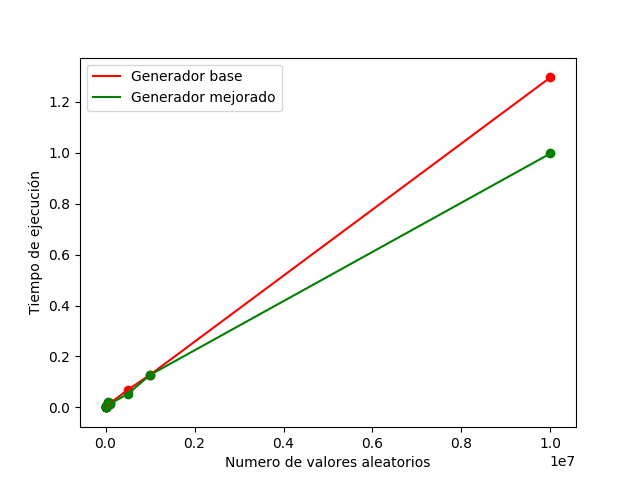
\includegraphics[scale=0.6]{img/mejora1.png}
\caption{Mejora de la distribución triangular reordenando la tabla.}
\label{fig:mejora1}
\end{figure}

Podemos ver que esta mejora permite reducir los tiempos de ejecución ligeramente a medida que va aumentando el número
de valores aleatorios, ya que modifica la estructura de la tabla para reducir los tiempos de la búsqueda lineal, al situar
los valores más probables primero. Sin embargo, el ``cuello de botella'' de este problema es la búsqueda, ya que sigue siendo
una búsqueda lineal, y por tanto, se irá recorriendo la tabla de forma secuencial hasta llegar al valor correcto.

\subsection{Mejorando la búsqueda: búsqueda binaria}

En esta segunda mejora vamos a modificar el algoritmo de búsqueda para ver si éste ofrece cierta mejora en general, y además,
si ofrece una mayor mejora comparándolo con solo reordenar la tabla.

Vamos a estudiar primero los resultados para las dos primeras tablas, comparándolos con los resultados base. Para el caso
de la tercera tabla, vamos a comparar también con los resultados de la sección anterior.

A continuación podemos ver los resultados para las dos primeras tablas:



\subsection{Tiempo de acceso constante a la tabla}

\section{Generadores congruenciales lineales}

\newpage

\begin{thebibliography}{5}

\bibitem{nombre-referencia}
Texto referencia
\\\url{https://url.referencia.com}

\end{thebibliography}

\end{document}

